\chapter{研究现状和相关工作}

视频流媒体的研究可以从系统模块(参见图\ref{fig:01})的角度分为几个方面:一是数据源端,包括如何提高视频编码的压缩率,如何支持码流的可伸缩性;二是传输过程,包括如何改善网络状况,如何充分合理利用带宽资源;三是客户终端,包括如何快速解码和更好的显示。本章首先对视频编码和传输领域的研究状况进行综述,然后结合本文所涉及的研究内容,对相关的问题和已有工作进行分析。

\begin{figure}[h]
	\centering
	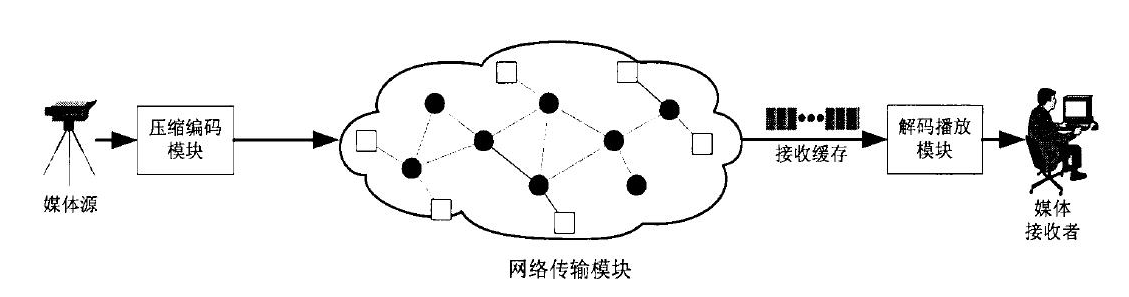
\includegraphics[width = 0.9\linewidth]{clip/01.png}
	\caption{流媒体系统模块 \label{fig:01}}
\end{figure}

\section{视频的压缩编码}

原始视频信号数据量过于庞大,必须经过压缩才能有效进行存储和传输。视频信号之所以能被压缩是因为其中存在大量冗余信息,包括空间冗余、时间冗余、统计冗余等\supercite{Gao-book-2010}。以仙农信息\supercite{Shannon-1948}论和率失真理论\supercite{Berger-book-1984}为基础,通过预测(如时间预测和空间预测)\footnote{在空域或时域寻找相似信号,用与相似信号的残差来重建当前信号的一种压缩手段}、变换(如离散余弦变换\supercite{Rao-1990}、哈达玛变换\supercite{Pratt-1969})、量化\supercite{Gray-TIT1997}、熵编码(如变长编码\supercite{Huffman-1952} 、算术编码\supercite{Rissanen-1979})等技术手段,可以去除这些冗余,以一定的失真为代价获得很高的数据压缩比。数字视频压缩编码技术经过了半个多世纪的发展,形成了一系列的国际标准。

最早的视频编码标准通常被认为是由国际电信联盟(ITU)于1990年制定的H.261\supercite{H.261}。同一时期,由国际标准化组织和国际电工委联合成立的运动图像专家组(MPEG)也开始了视频相关标准的制定工作,并于1992年推出了MPEG-1\supercite{MPEG1}。此后,以MPEG-2\supercite{MPEG2}、H.263\supercite{H.263}为代表的标准不断演进,大大推动了数字视频产业的发展。时至今日,国际电信联盟与国际标准化组织已经在标准制定方面互相合作,二者共同打造的H.264/AVC视频编码标准\supercite{H.264}在蓝光光碟、高清DVD、数字电视广播、互联网视频共享和在线观看等各个领域都占据了主流地位,普及度极高。虽然意在取代H.264/AVC的新一代视频编码标准HEVC已经于2013年发布,但因为其编解码复杂度高且大多设备和系统尚未支持,所以还处于推广阶段。我国也制定了自己的视频编码标准AVS (Audio Video coding Standard) \supercite{AVS},但影响力远不及国际标准。考虑到上述情况,我们的研究大部分都是基于H.264/AVC及其扩展的;针对新一代视频编码标准HEVC的解码器优化也正是为了促进其推广应用。

下面对H.264/AVC视频编码标准和它的扩展之一——可伸缩视频编码进行介绍,作为后文工作的基础。

\subsection{H.264/AVC视频编码标准}

H.264/AVC的设计目标有两方面,一是显著提高编码效率,二是在网络化的趋势下满足对灵活性和可定制性的要求。为此,这一新标准提出了两个概念:视频编码层(Video Coding Layer,VCL)用于高效的表示视频内容,而网络抽象层(Network Abstract Layer,NAL)则封装视频的VCL表示并提供头部信息,使之适用于多样化的传输层次和存储介质(参见图\ref{fig:02}\supercite{H.264-Overview})。

\begin{figure}[h]
	\centering
	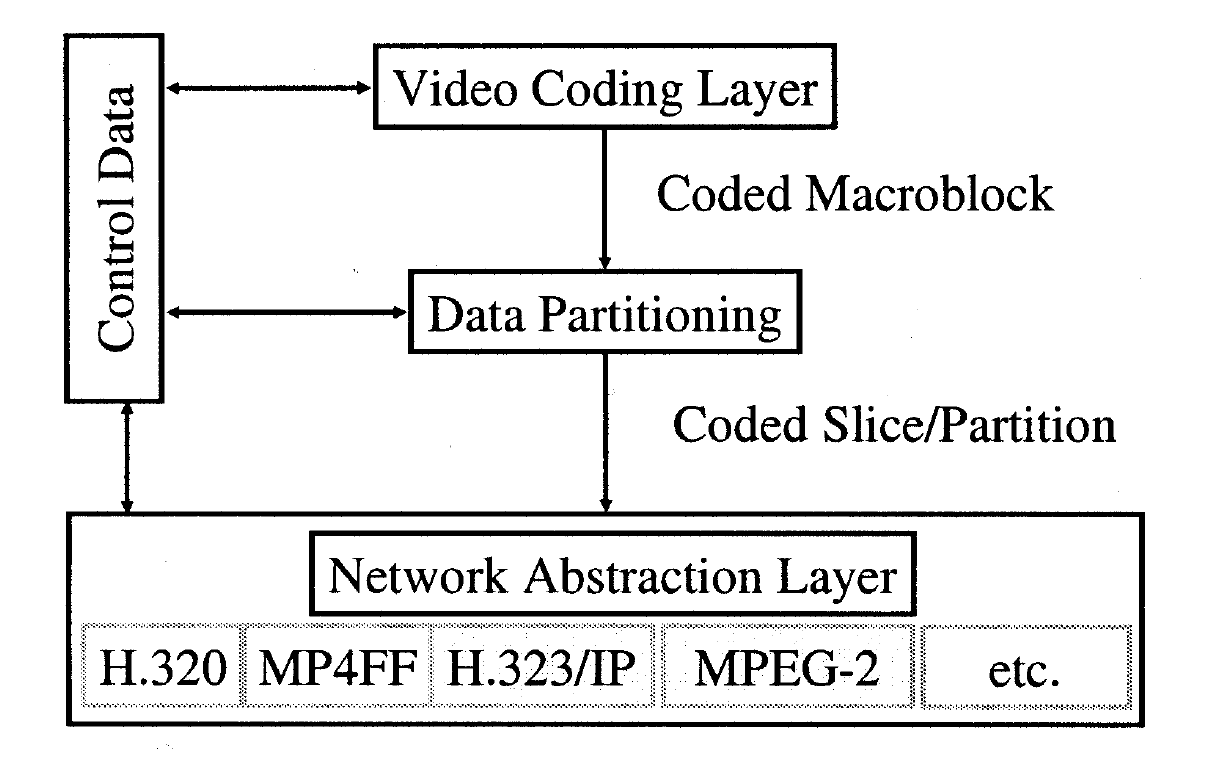
\includegraphics[width = 0.6\linewidth]{clip/02.png}
	\caption{H.264/AVC编码标准的结构\label{fig:02}}
\end{figure}

图\ref{fig:02}中,H.320是国际电信联盟制定的关于在ISDN(综合数字交换网)上进行视频会议的标准,H.323则是其在IP电话方面的标准,MPEG-2规定了音视频文件存储格式。可见,经过NAL层的抽象,H.264/AVC编码得到的码流可以灵活适应各种应用。下面,分别对VCL和NAL进行介绍。

VCL层的目标是高效率地表示视频内容。与其他视频编码标准一样,H.264/AVC的VCL层采用了基于块的混合视频编码框架,如图\ref{fig:03}所示。

\begin{figure}[h]
	\centering
	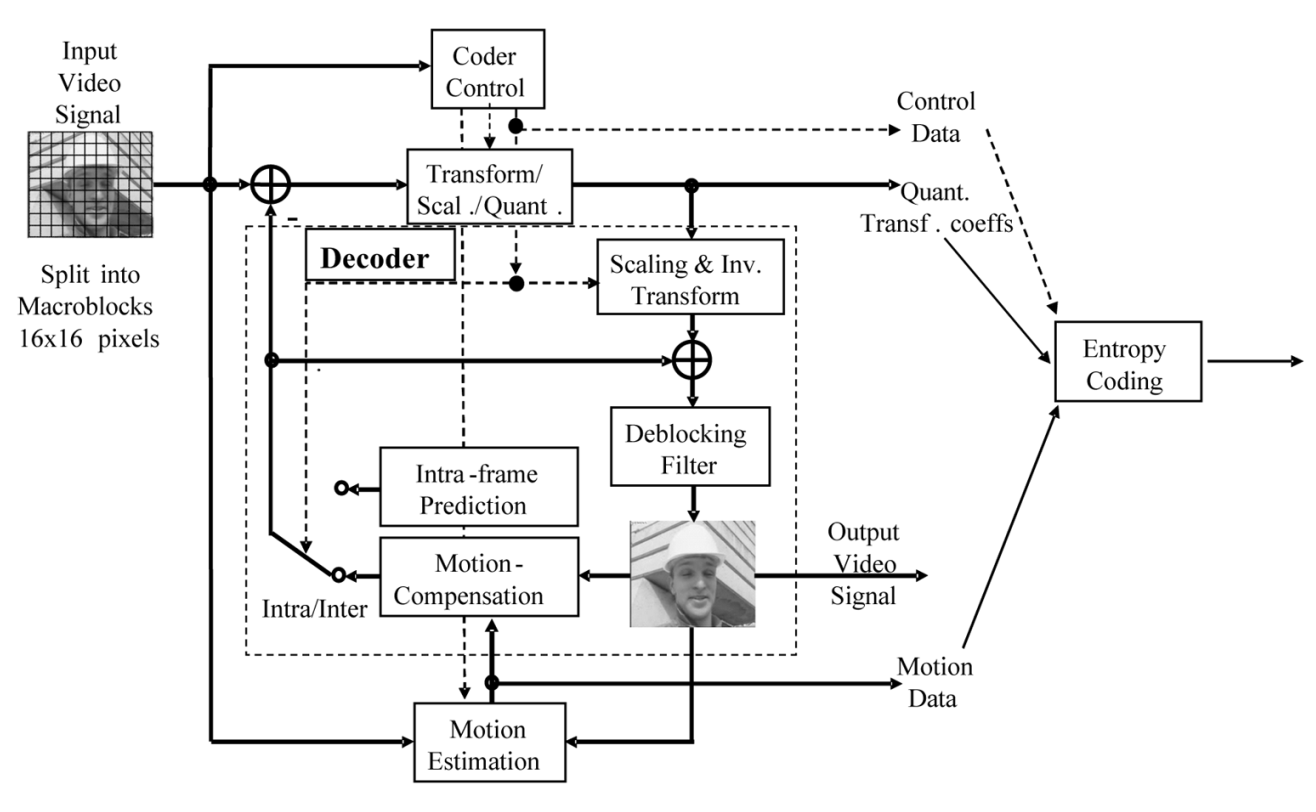
\includegraphics[width = 1.0\linewidth]{clip/03.png}
	\caption{H.264/AVC的VCL层编码框架\label{fig:03}}
\end{figure}

所谓“基于块”,是指将原始图像数据分成16x16大小的宏块(Macro Block,MB),接下来的编码过程将以宏块为基本单位。对每一个宏块,先进行时间或空间预测;预测得到的残差数据进行类似于DCT的整数变换,然后对变换系数进行量化、重排、熵编码,最终形成比特流。

虽然这样的编码流程与之前的编码标准并无二致,但由于H.264/AVC对各个阶段进行了精心设计,并将灵活性和适应性贯穿于整个编码过程,使得其编码效率大大提高。以下仅着重分析H.264/AVC相对于之前标准的改进之处。

预测分为帧内预测和帧间预测,目的分别是去除空间和时间冗余。在H.264/AVC中,预测时可将一个宏块进一步分为小的子块进行,最小可以分成4x4的小块。标准还提供了多达9种的预测模式,从而能够更精细地利用局域特性。而对帧间预测,H.264/AVC除支持单向和双向预测之外,每个方向还允许选用多个参考帧。在运动向量的准确度上,新的标准允许精确到1/4像素,而且还允许跨越边界的值(采用外推插值技术)。

对预测残差进行变换可以进一步去除空间相关性。考虑到精细的预测模式已经很好的去除了相关性,H.264/AVC一改之前标准以宏块为单位的DCT变换,采用了更小的变换块(4x4)。而且对于相对平滑的色度值(YCbCr/YUV中的U、V),还对每个宏块中的4个4x4子块变换后的直流系数又做了一次哈达玛变换。小尺寸块的变换大大减小了计算复杂性。当然,H.264/AVC也支持将变换块扩展成16x16大小。

H.264/AVC提供了两种熵编码方法CAVLC(Context Adaptive Variable Length Coding)和CABAC(Context-based Adaptive Binary Arithmetic Coding)来去除量化后系数(以及其他一些参数)的统计冗余。它们都是上下文自适应的,前者为可变长编码,后者为二进制算术编码,后者计算较复杂但压缩率高,前者反之,可根据应用场景配置不同的算法。

以上只选取VCL的部分特性进行了简述。除了所提到的方面,H.264/AVC还包含更多可由编码器选择的配置。这样不仅能够更有针对性地去除冗余、提高编码效率,而且也增加了该标准的普适性、灵活性和可定制性。正因为如此,能够在其基础上方便地进行扩展。

VCL编码得到的比特流送去NAL层进行封装。NAL的设计目标是提供网络友好性,使得VCL数据在不同系统中的使用可以简单而高效地定制。我们后面将看到,在H.264/AVC基础上扩展得到的码流能与普通的H.264/AVC码流无缝兼容,很大程度上得益于这种网络抽象层机制。

网络抽象层的基本概念和语法结构是NAL 单元(NAL Unit,NALU)。这是一种由整数个字节组成的数据包。一个NALU以1字节的头信息起始,之后是不定长度的载荷。参见表\ref{tab:nal}。

\begin{table}[h]
\centering
\caption{H.264/AVC中的NAL单元结构}
\label{tab:nal}
\begin{tabular}{*{11}{p{1.2cm}<{\centering}|}{p{1.2cm}<{\centering}}}
	\hline
	\multicolumn{8}{c|}{NALU头字节} & \multicolumn{4}{c|}{NALU载荷} \\ \hline
	F & \multicolumn{2}{c|}{NRI} & \multicolumn{5}{c|}{TYPE} & \multicolumn{4}{c|}{......} \\ \hline
\end{tabular}
\end{table}

NALU字节头包含禁止位 (F,1bit) 、重要性指示位 (NRI,2bit) 、NALU类型 (TYPE,5bit) 三方面信息。其中禁止位规定为0,重要性指示位在一定意义上表示该NALU的重要程度(或传输时的优先级),而NALU类型则表明该NALU的载荷类型。

在H.264标准中,NALU类型的0~12已用,13~23被保留用于以后可能的扩展(如SVC扩展用到了其中的值),24~31不做规定,可根据应用场景定制。按照NAL单元中载荷的不同,将其划分为两类:VCL 单元和non-VCL单元。前者主要包含来自VCL的图像样本值编码数据,后者主要含有图像或序列参数集、补充增强信息(Supplemental Enhancement Information,SEI)等解码多个VCL单元所共用的一些重要数据。这种机制不仅能节省开销,也便于将重要数据通过更可靠的信道传输。对如何使用SEI存储和传输数据,后文在码流截取部分会有涉及。

\subsection{可伸缩视频编码}

可伸缩视频编码(Scalable Video Coding,SVC),简言之,就是在视频编码时生成一个包含不同层次信息的码流。从这个单一码流中,我们能够方便地丢弃一些数据,得到不同码率的多个码流,从而解码出在空间大小、帧率、画面质量等方面可伸缩的视频。

基于H.264/AVC扩展而来的SVC在传统编码的基础上引入了“分层编码”的概念。即对数据源一次编码得到的码流中,含有一个或多个的“层”。其中最低分辨率、最低帧率和最差图像质量的部分称为基本层,除此之外为增强层。增强层对应着更高的分辨率、帧率和图像质量。这样的码流能够提供在空间、时间、质量(或SNR,即信噪比)等方面的伸缩性。当终端没有能力播放增强层或者网络无法承担高码率时,可伸缩码流的增强层部分会从比特流中移除,只有基本层数据被传送到终端解码器。SVC编码标准得益于H.264/AVC灵活的编码逻辑结构,也继承了H.264/AVC中许多良好设计的编码工具。SVC不仅在编码效率和复杂性上与单层编码增加不多\supercite{SVC-Performance},并且完全兼容H.264/AVC。可以预见,它将在未来的视频应用中成为主流。以下结合传统编码框架,在H.264/AVC的基础上,对SVC可伸缩性的实现原理进行概述。

具备时间可伸缩的码流能够根据需要动态改变视频帧率。在H.264标准中,把用于解码一帧的多个NAL单元称为一个AU(Access Unit)。SVC就是通过丢弃AU来降低帧率。时间可伸缩的实现不需要对H.264做任何增加,只需采用一种称为“层次化预测结构”的技术。

\begin{figure}[h]
	\centering
	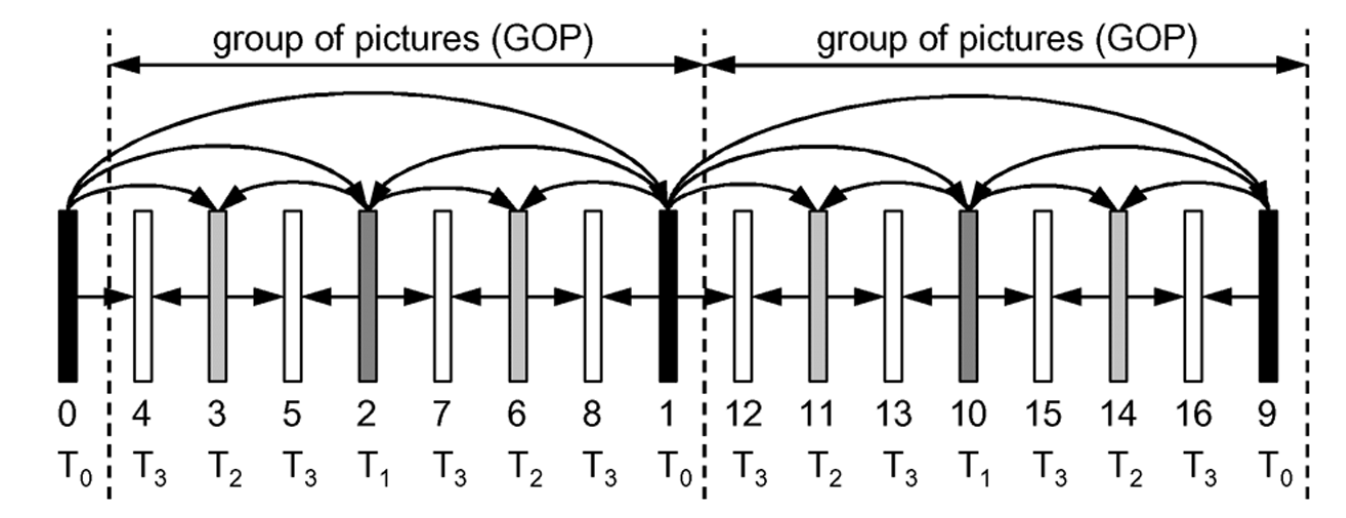
\includegraphics[width = 1.0\linewidth]{clip/04.png}
	\caption{H.264/SVC中通过层次化预测实现时间可伸缩\label{fig:04}}
\end{figure}

图\ref{fig:04}说明了通过层次化预测来实现时间可伸缩的原理。图中一个AU下面的数字表示其编码顺序,数字下面的符号Ti表示其属于第i时间层。增强层($i>0$)的帧被编码为B帧(即参考其前后的帧进行双向预测),而且只参考较低层的帧。这样的结构下,低层的AU可以不依赖于高层,即任一较高层及其以上各层的AU可以被丢弃而不影响解码,以此实现帧率的伸缩性。需要说明的是,此例中这种“层次化B帧”的结构会带来编解码时延,且仅限于1:2伸缩比,这些不足均可通过仔细设计层次化预测结构而改善。

空间可伸缩是指视频大小的改变。空间可伸缩的实现比较复杂,需要在H.264中引入分层编码。每个分辨率都对应一个H.264编解码层,称之为“dependency layer”,由DID(Dependency ID)标记。每个层都需要不同尺寸的输入图像,这一般由最高分辨率的图像下采样得到。每层的运动补偿和帧间预测都和单层H.264编码一样,然而由于表示的是同一图像,各层之间必然有很强的相关性。SVC规定了各层之间的预测机制,称之为“层间预测”,以此来提高编码效率。

质量可伸缩顾名思义就是视频各帧的图像质量可变。这是通过丢弃一个AU中的一些质量精细化NAL单元来实现的。具体操作时,给一个AU内的每个NAL单元打上质量层标记QID(Quality ID),可以将QID高于某个值的所有NAL单元丢弃,剩下的即可组成较低质量的码流。

以上分析的主要是在VCL层实现可伸缩编码的原理,可以看到多处涉及对特定NAL单元的取舍。这就需要对H.264的NAL层进行扩展从而能够在码流中标记和传送特定的可伸缩性信息与数据。

在前面介绍H.264/AVC时曾提到,NALU头字节中的NAL类型(nal\_type)在13~23的取值留作扩展;SVC就增加了一些扩展的NAL类型。nal\_type=20的单元为新增的VCL单元,包含的是SVC中增强层的编码数据;nal\_type=14为新增的SVC前缀单元,它可能是VCL的也可能是的non-VCL的,取决于紧接着它到来的NALU。此外,还有nal\_type=15的NALU来传送SVC特有的图像参数集。对于这些新增类型的具体分析可以参见相关文档\supercite{SVC-Interface}。

普通H264解码器遇到nal\_type大于12的单元会忽略之,但能成功解码基本层,因此SVC可与之兼容。而支持SVC的解码器将对类型为14、20的NALU进行利用,实现可伸缩性。与普通H.264的NALU不同,类型为14、20的NALU并非只有1个头字节,而是扩展为4字节的头。如图\ref{fig:05}所示。

\begin{figure}[h]
	\centering
	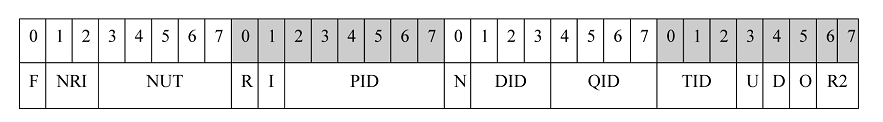
\includegraphics[width = 1.0\linewidth]{clip/05.png}
	\caption{4字节的SVC NAL单元头结构\label{fig:05}}
\end{figure}

可以看出,其中除了与普通NALU一致的第一字节,还包含了空间、时间和质量层的标志(DID、TID、QID)以及其他一些用于提供可伸缩性的信息。

根据以上分析,可在标准H.264编解码器的基础上扩展得到SVC编解码器。无论H.264还是SVC,在标准文档中都只对码流的语法语义和解码过程做了规定,换句话说:对编码的过程不做限制,只要得到符合标准的码流即可。因此编码器的程序实现可以多种多样,而解码必须与标准一致。
 
SVC标准由ITU与ISO的专家组成的联合视频小组(JVT)制定。该组织在标准形成后还发布了一个官方的参考软件,称为JSVM(Joint Scalable Video Model)\supercite{JSVM}。该软件完整实现了SVC的编解码过程。虽然该软件未做优化很难实用,但由于其囊括了SVC标准中的几乎所有特性且清晰逻辑、配置简单,比较适合学习参考,以及作为研究性的实验平台。因此,几乎所有的学术工作都是基于JSVM参考软件,在其上实现自己的算法并与内置的算法进行对比,体现其效率的提升。

H.264/AVC、SVC这些视频编码标准的制定和推广过程不仅促进了产业发展,还在以下两个方面产生了大量的研究工作:一是对信源编码理论的研究,二是对视频编码与网络传输相结合的应用技术的研究。

\section{视频的流式传输}

\subsection{互联网视频传输协议}

\subsection{代表性的流媒体服务器}


\section{可伸缩视频码流截取}

\subsection{问题描述}

所谓码流截取,是指从一个完整的码流中抽取所有数据包的一个子集,得到一个更低码率的子流的过程。图\ref{fig:Bitstream-Extraction}展示了一个可伸缩视频码流的结构,以及从中截取子流的一种可能的方式。
可以看到,该码流中的数据包被分为了不同的层。时间层(T0~T3)反映了各帧之间的参考或依赖关系。图形上方的箭头从被参考帧指向参考它(也就是依赖于它)的帧。质量层(Q0~Q2)反映了一帧之内的视频质量伸缩性。处于高层(也就是Q1和Q2层)的数据包可以被部分丢弃从而实现码流截取。图中的虚线表示了一个截取的例子。虚线上方的数据包全部被丢弃,只有虚线下方的数据包保留在截取出来的子流中。

\begin{figure}[h]
\centering
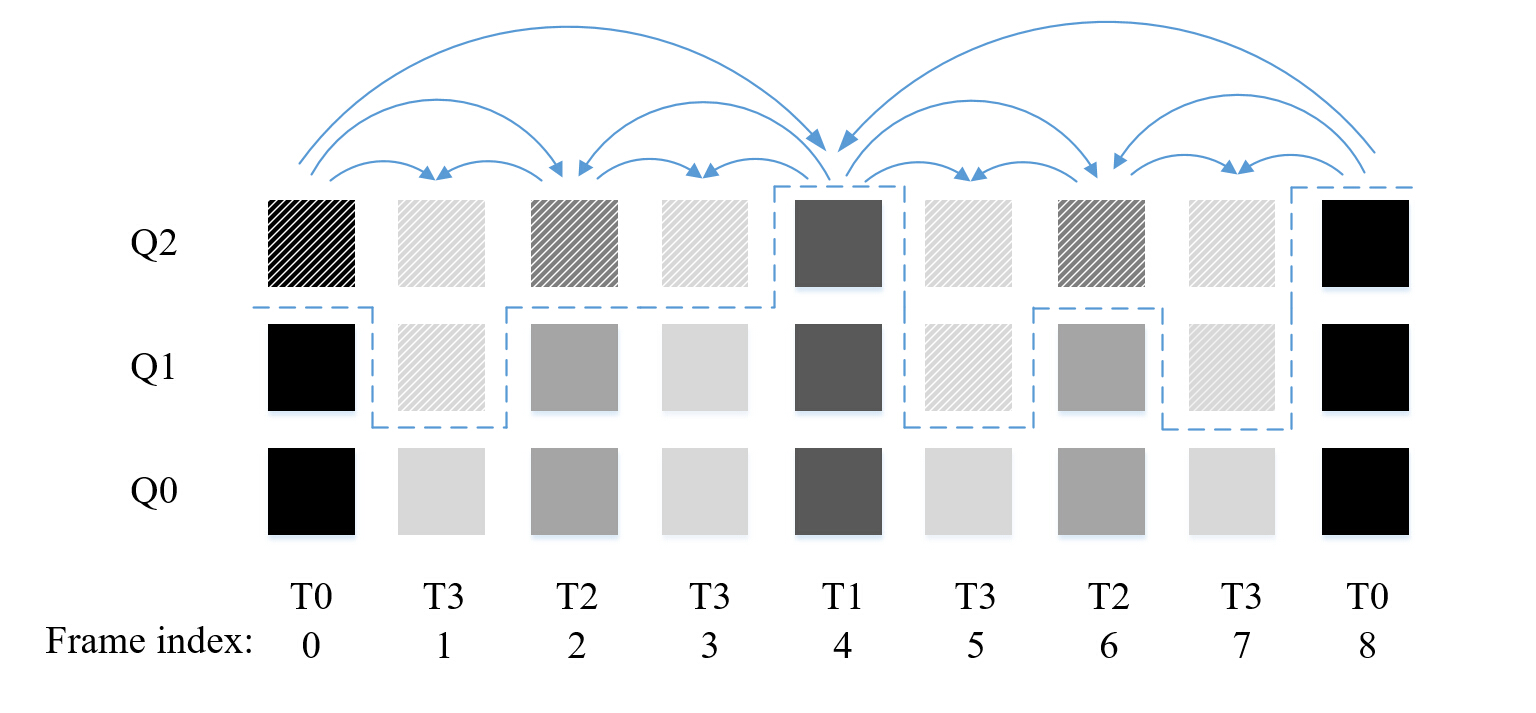
\includegraphics[width = 0.9\linewidth]{./figures/Bitstream-Extraction.jpg}
\caption{可伸缩视频码流截取 \label{fig:Bitstream-Extraction}}
\end{figure}

容易发现,可伸缩视频码流截取从本质上来看其实是一个组合优化问题。在所有的数据包中,我们希望在给定的码率限制下,选出一个最优的数据包组合,使得它们构成的子流具有最大的视频质量。更准确地说,这个问题与大家所熟知的“0-1背包问题”\footnote{http://en.wikipedia.org/wiki/Knapsack\_problem}在形式上是一致的。每个数据包可以看作是一个具有特定重量和价值的物品。这里的重量就是数据包的大小,价值就是它对重建视频质量的贡献。码流截取的过程就是决定每个数据包是否包含在最终的子流里。用“0-1背包问题”中的术语来说,就是选择将哪些物品放入背包中。

对于典型的“0-1背包问题”而言,其最优解可以用动态规划的方法得到。然而对于码流截取问题来说,这个方法是不可行的。主要原因在于数据包之间的依赖关系。首先,截取的数据包子集不能任意挑选,因为如果一个包被包含进了子流中,那么这个包所依赖的数据包也必须被包含进去,否则将无法正确解码。例如,在图\ref{fig:Bitstream-Extraction}中,我们不能只选择一帧中的Q2层数据包而丢弃同一帧的Q1层。其次,不同于“0-1背包问题”中定义良好的物品价值,码流截取问题中一个数据包对最终视频质量的贡献并不是明显且确定的。这是因为,数据包所在的帧在解码中是互相参考的,它们对视频质量的影响会互相干扰,对于不同的截取方案,每个数据包的实际贡献可能有所不同。事实上,除非实际进行一遍截取、解码、计算的操作,我们甚至无法准确地得到所截取出的子流的真实视频质量。这就使得可伸缩视频码流截取问题成为了一个复杂得多的问题。

\subsection{相关工作简介}

就我们所知,学术界没有人提出过一种确定能找到码流截取最优解的方法。当然可以用暴力穷举的方法来解决这个问题,但其复杂度显然是无法接受的。相关的工作都是尽可能用较低的计算量获得较好的次优解。下面对可伸缩视频码流截取的相关工作做简要的介绍。

最初的参考软件JSVM提供了一个非常简单的基本截取器。该截取器并没有考虑任何优化,只是实现了一个从完整码流中丢弃一些层的包来使码率低于给定值的程序。该程序按照SVC中的层的概念将所有NAL数据包分成了几组,在截取丢包的时候,高层的包先丢,如果整个高层都丢弃之后仍然不能满足码率要求,再考虑丢低层的数据包。这种方法符合直观理解,因为一般来说低层的数据作为被参考对象,影响的范围更广,重要性更大一些,所以应该优先保留;反之,高层的数据可以先丢。但编码过程中形成的数据包之间的关系并没有这么简单,有可能某个高层的包比某个低层的包更重要,基本截取器并没有考虑这一点。因此,基本截取器的效果离最优还有很大的差距。此外,对于同一个层的数据包,基本截取是按某个固定的顺序依次丢弃,也并没有对这些同一层数据包的重要性做区分。这也是基本截取器效率低下的另一个原因。接下来介绍对基本截取器的改进工作。

Amonou等人\supercite{Amonou2007}提出了一个基于“Quality Layers”的码流截取方案。这一方案被SVC参考软件JSVM所采用,而且取得了比JSVM中的基本截取器更好的性能。在Amonou等人的方案中计算了一个“Quality Layers”(简称QL)值,它反映了一个数据包的码率失真影响,据此进行截取能得到率失真优化过的结果。对于计算出来的QL值,可以用两种方法将其存储在码流中:

\begin{itemize}
\item 占用NALU头信息中的priority\_id字段来存储这个NALU的QL值。这个字段有6比特,只能存储64个不同值;
\item 用专门的补充增强信息(SEI)数据包来存储所有NALU的QL值。
\end{itemize}

在计算QL值的时候,对数据包失真影响的估计是一个计算量非常大的过程,而且估计的准确性也有提高的空间。因此,后续工作提出的失真模型一方面是降低复杂度,另一方面是进一步提高准确度。Sun等人\supercite{Sun2009}和Maani等人\supercite{Maani2009}所构造的模型都是基于帧间的误差漂移来计算失真。Sun等人的模型在性能方面几乎与JSVM相当,但计算复杂度却大大减少。而Maani等人的模型取得了比JSVM更高的估计准确度,但是由于其是基于训练的,为了得到更鲁棒的模型参数,需要更大的计算量。

Ramanathan等人\supercite{Ramanathan2012}提出了一个“Quality Metadata”的概念来用于码流截取,这与上面所说的“Quality Layers”是同样的思想,只是计算方法有所差别。Yang等人\supercite{Yang2013}提出了一个基于模拟退火的方法来解决码流截取问题。因为码流截取从另一个角度看是丢弃数据包的过程,丢弃的先后顺序可以认为是这些数据包的优先级。于是一些研究者从赋优先级的角度来提出相应的算法。例如,Lim等人\supercite{Lim2006}把可伸缩视频码流视为树形结构并据此来为每个数据包赋予优先级,而Zhu等人\supercite{Zhu2011}则采用拉格朗日乘子方法计算优先级值。在这些已有的工作中,失真估计的准确性都显著地影响最终结果。因此,提出简单有效的误差或失真模型对于码流截取的研究至关重要。本文的研究工作正是在此处着力并取得了创新性成果。


\section{传输中的码率自适应}

\subsection{问题描述}

在数据源具备码率可变的前提条件之后,实际传输时就可以根据带宽来调整发送的速率。改变码率去适应带宽的变化,这就是所谓的码率自适应问题。对于一个码率自适应算法,有三个最基本的目标。这三个目标可以用来衡量自适应算法的效果,也是设计算法时需要考虑的方面。下面分别进行描述。

对于一个流媒体系统,最首要的目标应该是保证视频播放能够连续不断。一旦视频开始播放,每个数据包都有了自己的显示时间。这个时间也决定了传输的截止时间。如果这个数据包没有在截止时间前达到客户端,那么客户端播放器就会因缺少数据而暂停。这就是用户所遇到的卡顿现象,应该努力避免。避免卡顿一般要依赖于传输中的缓冲机制。如果检测到带宽下降、当前码率确实过高,应及时下调质量,以防止数据不能按时传送而导致播放卡顿。

其次是要保持视频质量的平滑性。网络条件变化可能比较剧烈,但视频质量应该尽可能维持在一个比较稳定的水平。因为频繁的质量调整会给用户带来反感。举例来说,当用户适应了较低的质量后,突然调高质量并在短时间内又调低,给用户的体验还不如不调整。因此,在保证播放连续的前提下,应尽可能减少质量调整次数,充分利用缓冲区的作用,避免因为临时或短暂的带宽变化就调整质量。

最后,还要提供给用户尽可能好的视频质量。假设我们一直发送较低码率的视频流,那么既能保证播放的连续性又不存在平滑性的问题,上述两个目标可以轻而易举达到。但是这样的话用户看到的视频质量将一直处于较低的水平,显然不是令人满意的选择,所以不可取。码率自适应算法应该能够充分利用可用带宽,在带宽足够的情况下提高发送质量,给用户最好的观看体验。

综上所述,在视频流媒体的码率自适应研究中,保证播放流畅是最基本的要求,同时视频的高质量和平滑性也是所追求的指标。

\subsection{相关工作简介}

码率自适应的研究主要集中于如何选择和调度视频数据包。Gao等人\supercite{Gao2006}提出的调度策略首先确保重要性较高的数据优先发送,而对于重要性相同的数据包,播放时间最早的首先发送。Schier等人的工作\supercite{Schierl2010}也与此类似,把视频数据放在具有不同优先级的缓冲区中,通过调整优先级来确保数据及时发送。在Darwin流媒体服务器中内置有一个被称为包延迟反馈的调度算法。当一个包要发送时,DSS会检测它的延时(即这个数据包应播放的时间和当前时间的差),并根据这个延时来判断当前发送顺畅还是阻塞,以此来推测带宽情况,并相应调整发送码率和质量。具体判断方法是将这个延时作为反馈,与预先设定的阈值进行比较。例如,预先决定当前带宽下发送某个数据包之后T时间内应该播放,那么理想延时应该保持为T。如果发现延时小于T了,说明发送受阻,可能是带宽减小了;反之,如果T变大了,说明发送顺畅,可以考虑增加质量。这种算法能够在一定程度上检测带宽的变化并作相应调整。但是它的调整策略是保守的,在它检测到延时变小时,很可能客户端已经因为缺少数据而停止了。而且该算法对带宽的变化趋势也不能提前预测,很可能导致质量波动,这也是需要改善的一个问题。

上面的工作都是针对可伸缩视频流媒体系统或是RTSP传输协议进行的。近年来具有代表性的视频自适应传输方案是基于HTTP的动态自适应流媒体(DASH)\supercite{Sodagar2011}。DASH系统在服务器端提供不同码率的多个码流切片,客户端通过HTTP协议拉取数据,在某个时间段内可以选择性地接收这几个码流中任何一个的切片,通过在多码流之间切换来动态适应带宽波动。这就涉及如何制定码率调整策略,即码率自适应算法的设计。国内外对此已经有了不少研究。例如,Akhshabi等人\supercite{Akhshabi2012}分析了来自商业公司和开源社区的多个DASH客户端播放器的自适应行为,比较了他们之间性能的优缺点。张辉帅等人\supercite{Zhang2013}提出了一种基于拉模式的码率自适应算法,利用滑动窗口分析最近若干分片的下载时间,基于此来选择最合适的码流。Huang等人\supercite{Huang2015}结合了缓冲区的状态和对带宽容量的估计这两个判据来做如何调整码率的决策。Juluri\supercite{Juluri2015}等人考虑到每个分片数据量大小不同可能导致下载时间的差异,因此提出了一种提前查看分片信息的码率自适应算法。

这些已有的研究工作在一定程度上提高了传输效果,但大都是针对点播模式,没有考虑到直播模式下的特殊问题。目前实时性直播的应用越来越广,从某种程度上来说是一个更重要的模式。直播由于其数据是实时产生的,无法提前加载,因此与点播有所不同,需要进行针对性的研究,设计新的码率自适应算法。本文的工作不仅适用于点播系统,也能很容易应用到直播系统中。

\section{HEVC解码优化}

视频解码器优化的工作总是紧密结合视频编码标准而进行。在新一代国际视频编码标准HEVC推出以来,不少论文都针对其解码器实现和优化进行了研究。大部分已公开的研究工作都是在标准化组织所提供的参考软件HM\supercite{HM}的基础上进行的。在HM之外,我们所能查到的在正式发表文献中提出的独立解码器实现只有少数几个\supercite{Bossen-TCSVT2012,JCTVC-G988,JCTVC-H0693}。除了外在的性能报告和复杂度分析,这些文献中既没有给出任何技术细节或者源代码,也没有提供可以公开测试的演示程序。因此它们对HEVC的实际应用贡献并不大。Chavarrias等人\supercite{Chavarrias-TCE2013}提出了一个新的基于数字信号处理器(DSP)的HEVC解码器。但由于不是针对通用处理器平台,其应用局限性也比较大。本文主要关注的是在x86和ARM架构的通用处理器上的解码优化。下面分数据级和任务级两个方面对相关的工作进行介绍。

\subsection{数据级优化工作}

数据级解码器优化主要是采用单指令多数据(single-instruction-multiple-data,简称SIMD)的处理器指令集扩展来对解码过程中的特定计算模块进行加速。SIMD所适用的主要是运动校正、整数变换、去块滤波这些计算密集而规整的模块。不同编解码标准对这些模块的定义并不完全相同。就HEVC而言,它在运动校正时采用了8抽头的基于DCT的插值\supercite{JCTVC-F537},而且在去块滤波之后加入了一个称为采样自适应偏移(sample adaptive offset,简称SAO)的新操作\supercite{Fu-TCSVT2012}。由于SIMD算法的设计与这些模块的操作密切相关,因此针对以前标准设计的数据级解码优化算法\supercite{Casalino-ICMCS1999,Lappalainen-TCSVT2003,Malvar-TCSVT2003,Chen-JVCIR2006,Pescador-TCE2009}都不再适用于HEVC。Yan等人\supercite{Yan-VCIP2012}在HM 4.0的基础上,采用SIMD技术对一些解码模块进行了加速。但随着标准文档和参考文件的更新,最终版本的HEVC相对于HM 4.0有些模块发生了变化,例如上述工作中所加速的自适应滤波\supercite{JCTVC-F303}最终被从标准中移除。因此,针对最新的标准需要重新设计和实现数据级的优化算法。

\subsection{任务级优化工作}

任务级解码器优化主要是通过多线程来并行执行解码任务,以充分利用多核CPU的并行特性。HEVC标准在设计的时候考虑了对任务级并行的支持,引入了分片(tiles)\supercite{JCTVC-E408}和波阵面并行处理(wavefront parallel processing,简称WPP)\supercite{JCTVC-E196}这两种技术。它们能够将解码分成互相独立的任务来同时执行,一定程度上可以提高整体解码速度。Chi等人\supercite{Chi-TCSVT2012}还基于WPP提出了一个称为“overlapped wavefront”的任务级并行优化技术,对于用WPP编码的视频码流取得了期望的解码加速比。然而需要指出的是,分片和WPP都是HEVC标准中的可选配置,如果视频码流在编码的时候没有开启这些选项,那么解码器就无法利用这两个新特性。从实用的角度来看,采用不依赖于这些特殊配置的帧级并行解码结构才具有更广泛的意义。这也正是本文工作所选择的方向。

\section{本章小结}

本章从分析视频流媒体的系统模块入手,首先对该领域的研究状况以及视频编解码和传输技术做了介绍,其中包含了本文研究工作的知识基础;然后结合本文的研究内容对码流截取、码率自适应、解码器优化这几个方面的问题和已有工作进行了概述。后续章节将对这几个方面依次进行研究。